\documentclass{cumcmthesis}
\usepackage[framemethod=TikZ]{mdframed}
\usepackage{graphicx}
\usepackage{url}   % 网页链接
\usepackage{subcaption} % 子标题
\usepackage{booktabs} % 浮动体
\usepackage{amsmath}
\usepackage{svg}
\usepackage{listings}

\title{我的论文标题}
\tihao{C}
\baominghao{121}
\schoolname{上海交通大学}
\membera{张航}
\memberb{刘允禾}
\memberc{高慧鑫}
\supervisor{高晓沨}
\yearinput{2026}     % 年
\monthinput{09}      % 月
\dayinput{13}

\begin{document}

\maketitle

\begin{abstract}
            
            \keywords{关键词1\quad  关键词2\quad   关键词3}
        \end{abstract}
        \section{问题重述}
        \subsection{问题背景}
        在生鲜商超中，蔬菜作为主要的生鲜商品之一，其销量的变化直接影响到商超的经营效益。然而，蔬菜类商品的保质期较短，且品相随销售时间的增加而变差。因此，了解蔬菜的销售规律，根据历史销售数据和需求情况制定补货量和定价策略尤为重要。
        \subsection{问题重述}
        本研究结合所提供的销量数据，旨在通过数据分析和建模方法，解决以下四个问题：
        \newline
        \quad\textbf{问题一:}分析数据，研究各品类蔬菜及各单品销量随时间的分布规律和相互关系。
        \newline
        \quad\textbf{问题二:}
        \newline
        \quad\textbf{问题三:}
        \newline
        \quad\textbf{问题四:}
        \section{问题分析}
        \subsection{问题一的分析}
        问题一并未明确指出具体的分析目标，考虑到销售量的分布规律可能分为按时间分布、按订单数量分布、按蔬菜品类分布，我们将分析目标定为研究各品类蔬菜及单品的销售量在一年、一个星期和一天内的分布规律；此外，相互关系可分为各品类蔬菜销量的相互关系和各单品销量之间的关系。为此，我们将对数据进行时间序列分析，使用统计方法和可视化工具来揭示销售量的趋势、季节性和周期性特征。同时，我们将计算各品类蔬菜及单品之间的相关系数，以了解它们之间的相互关系。
        \subsection{问题二的分析}
        \subsection{问题三的分析}
        \section{模型假设}
        1.假设各蔬菜品类及单品的市场需求不受市场竞争的影响。\newline
        \hspace*{2em}2.假设蔬菜的销售量与价格之间存在一定的关系，且该关系在一定时间范围内保持稳定。\newline
        \hspace*{2em}3.假设假设各商品之间的需求关联仅存在于同一销售周期内，不考虑“今日未购买则明日补购”的跨期替代效应。
        \section{符号说明}
        \begin{center}
            \begin{tabular}{cc}
                \hline
                \makebox[0.3\textwidth][c]{符号}	&  \makebox[0.4\textwidth][c]{意义} \\ \hline
                D	    & 木条宽度（cm） \\ \hline
            \end{tabular}
        \end{center}
        \section{数据预处理}
        \subsection{异常数据处理}
        通过分析附件发现存在缺失值，我们将其视为无效数据并予以剔除。对于因退货导致销售额小于零的数据，其对研究销售分布规律无益处，也予以剔除。对于附件1里有、但附件2中没有任何销售记录（无销量）或销售天数过少（$\leq 10$天）、销售占比过小（$\leq0.00003$）的单品，予以剔除。
        \begin{figure}
    \centering
    \begin{minipage}[c]{0.48\textwidth}
        \centering
        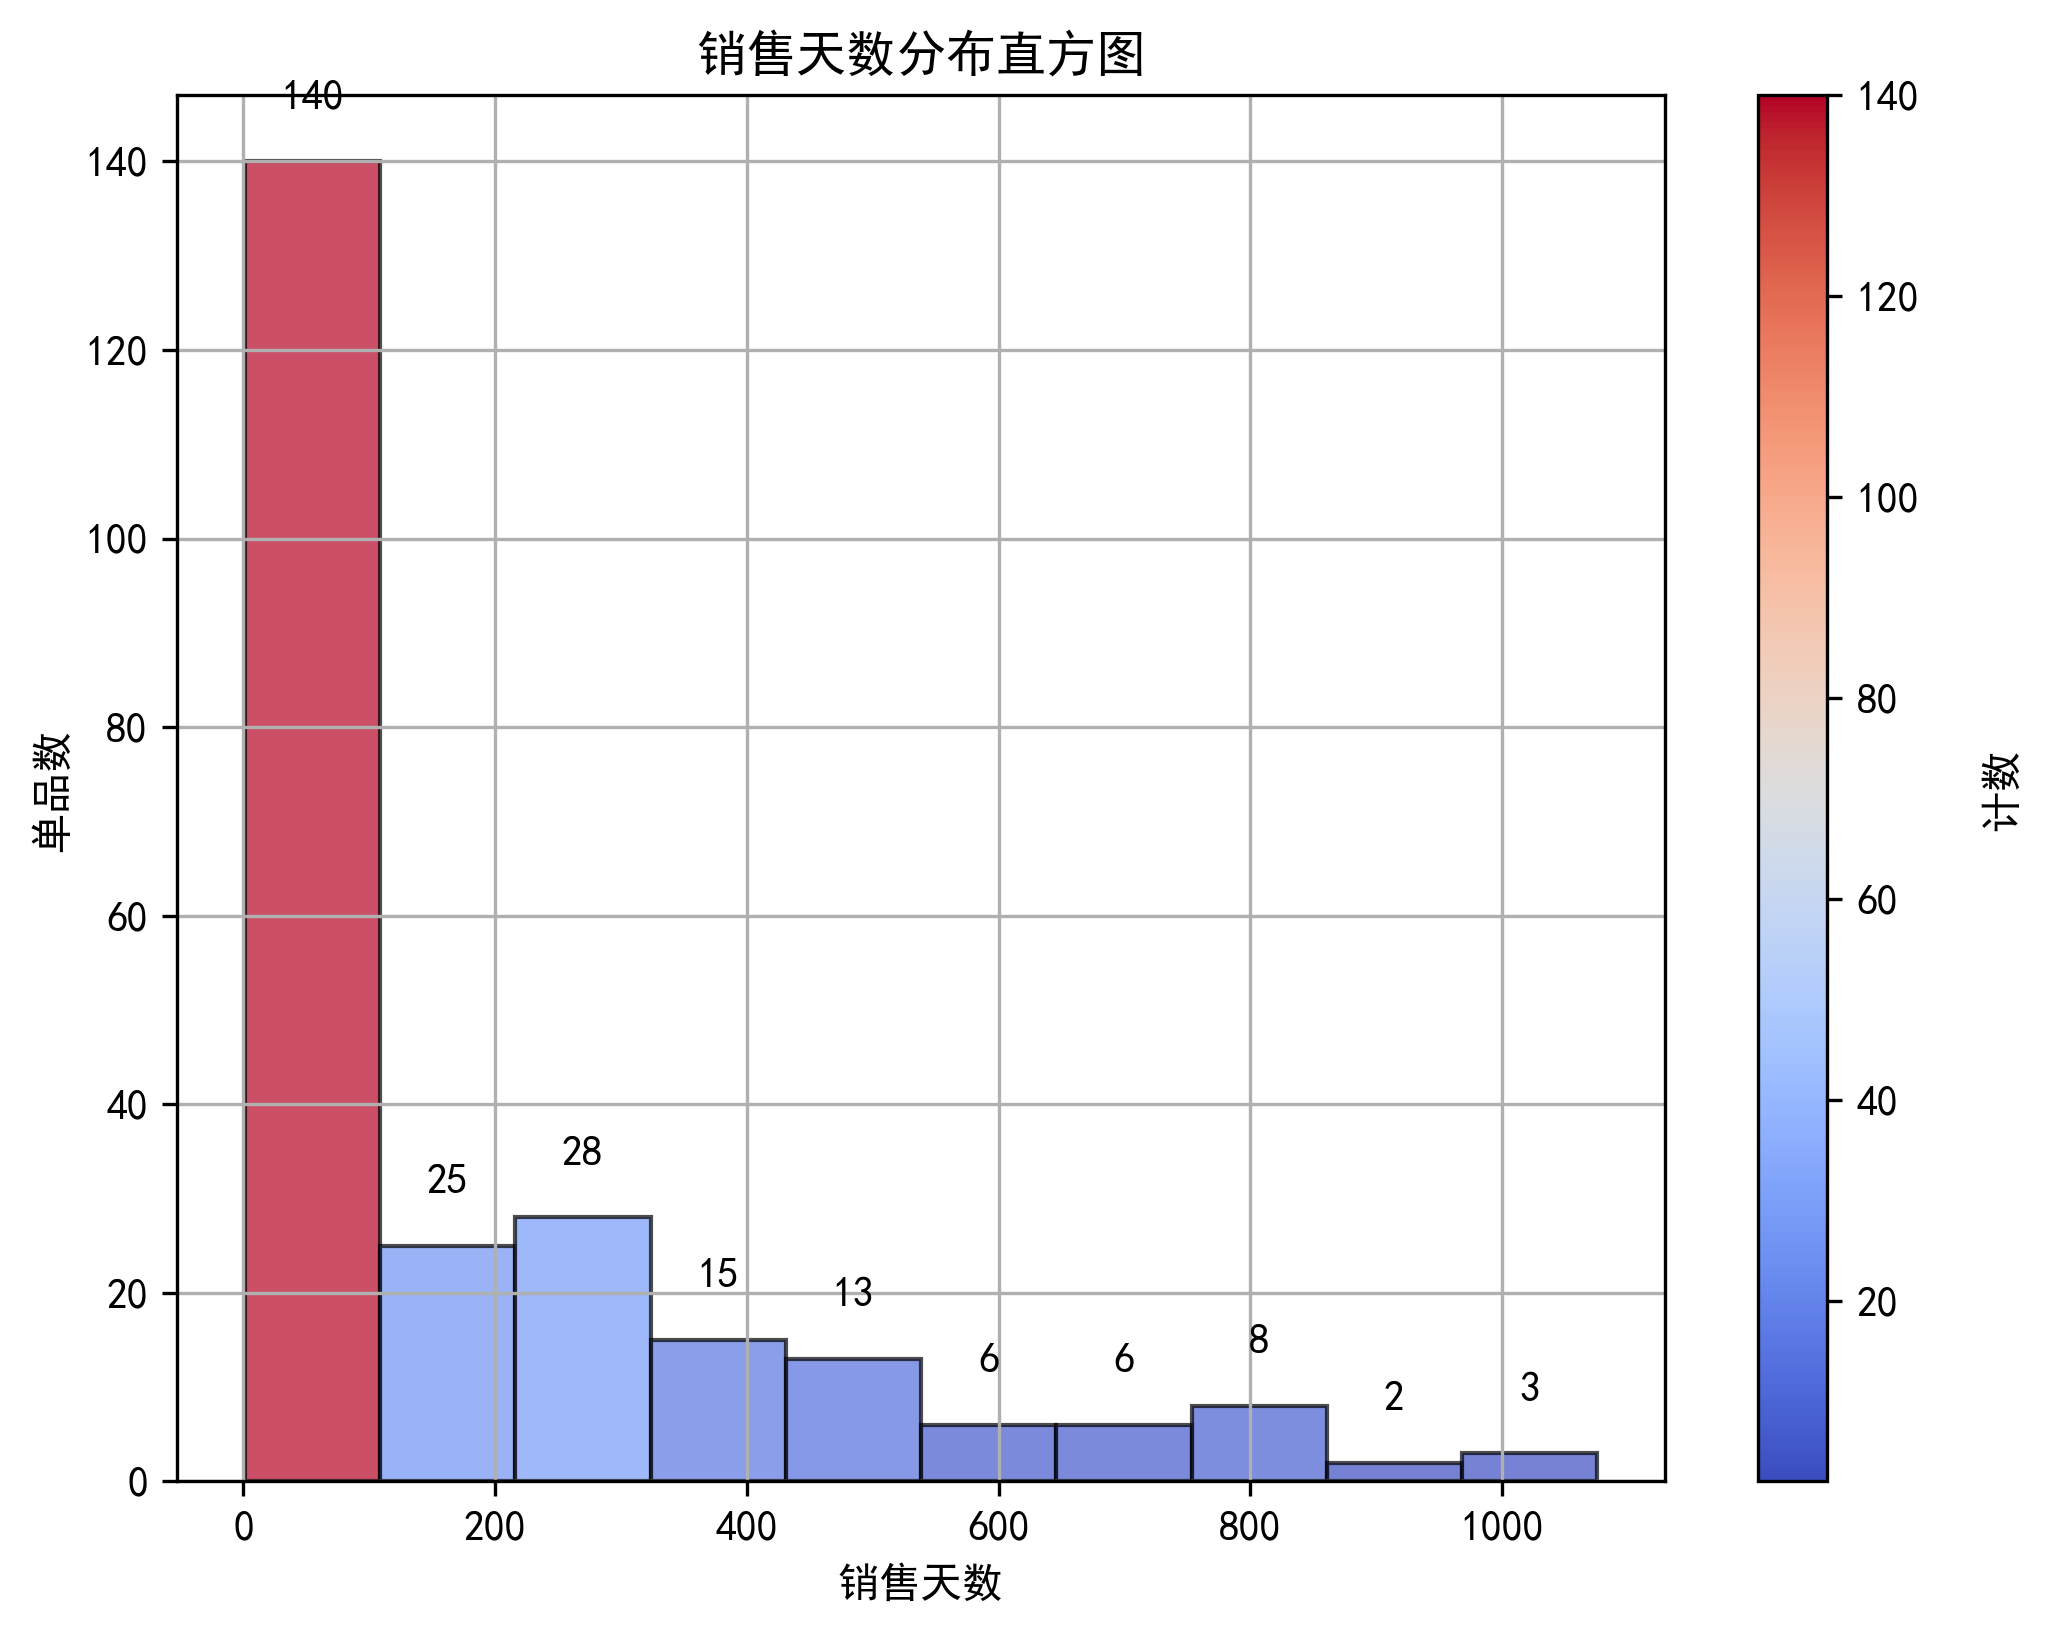
\includegraphics[width=0.95\textwidth]{销售天数直方图.png}
        \subcaption{销售天数直方图}
        \label{fig:sample-figure-a}
    \end{minipage}\hfill
    \begin{minipage}[c]{0.48\textwidth}
        \centering
        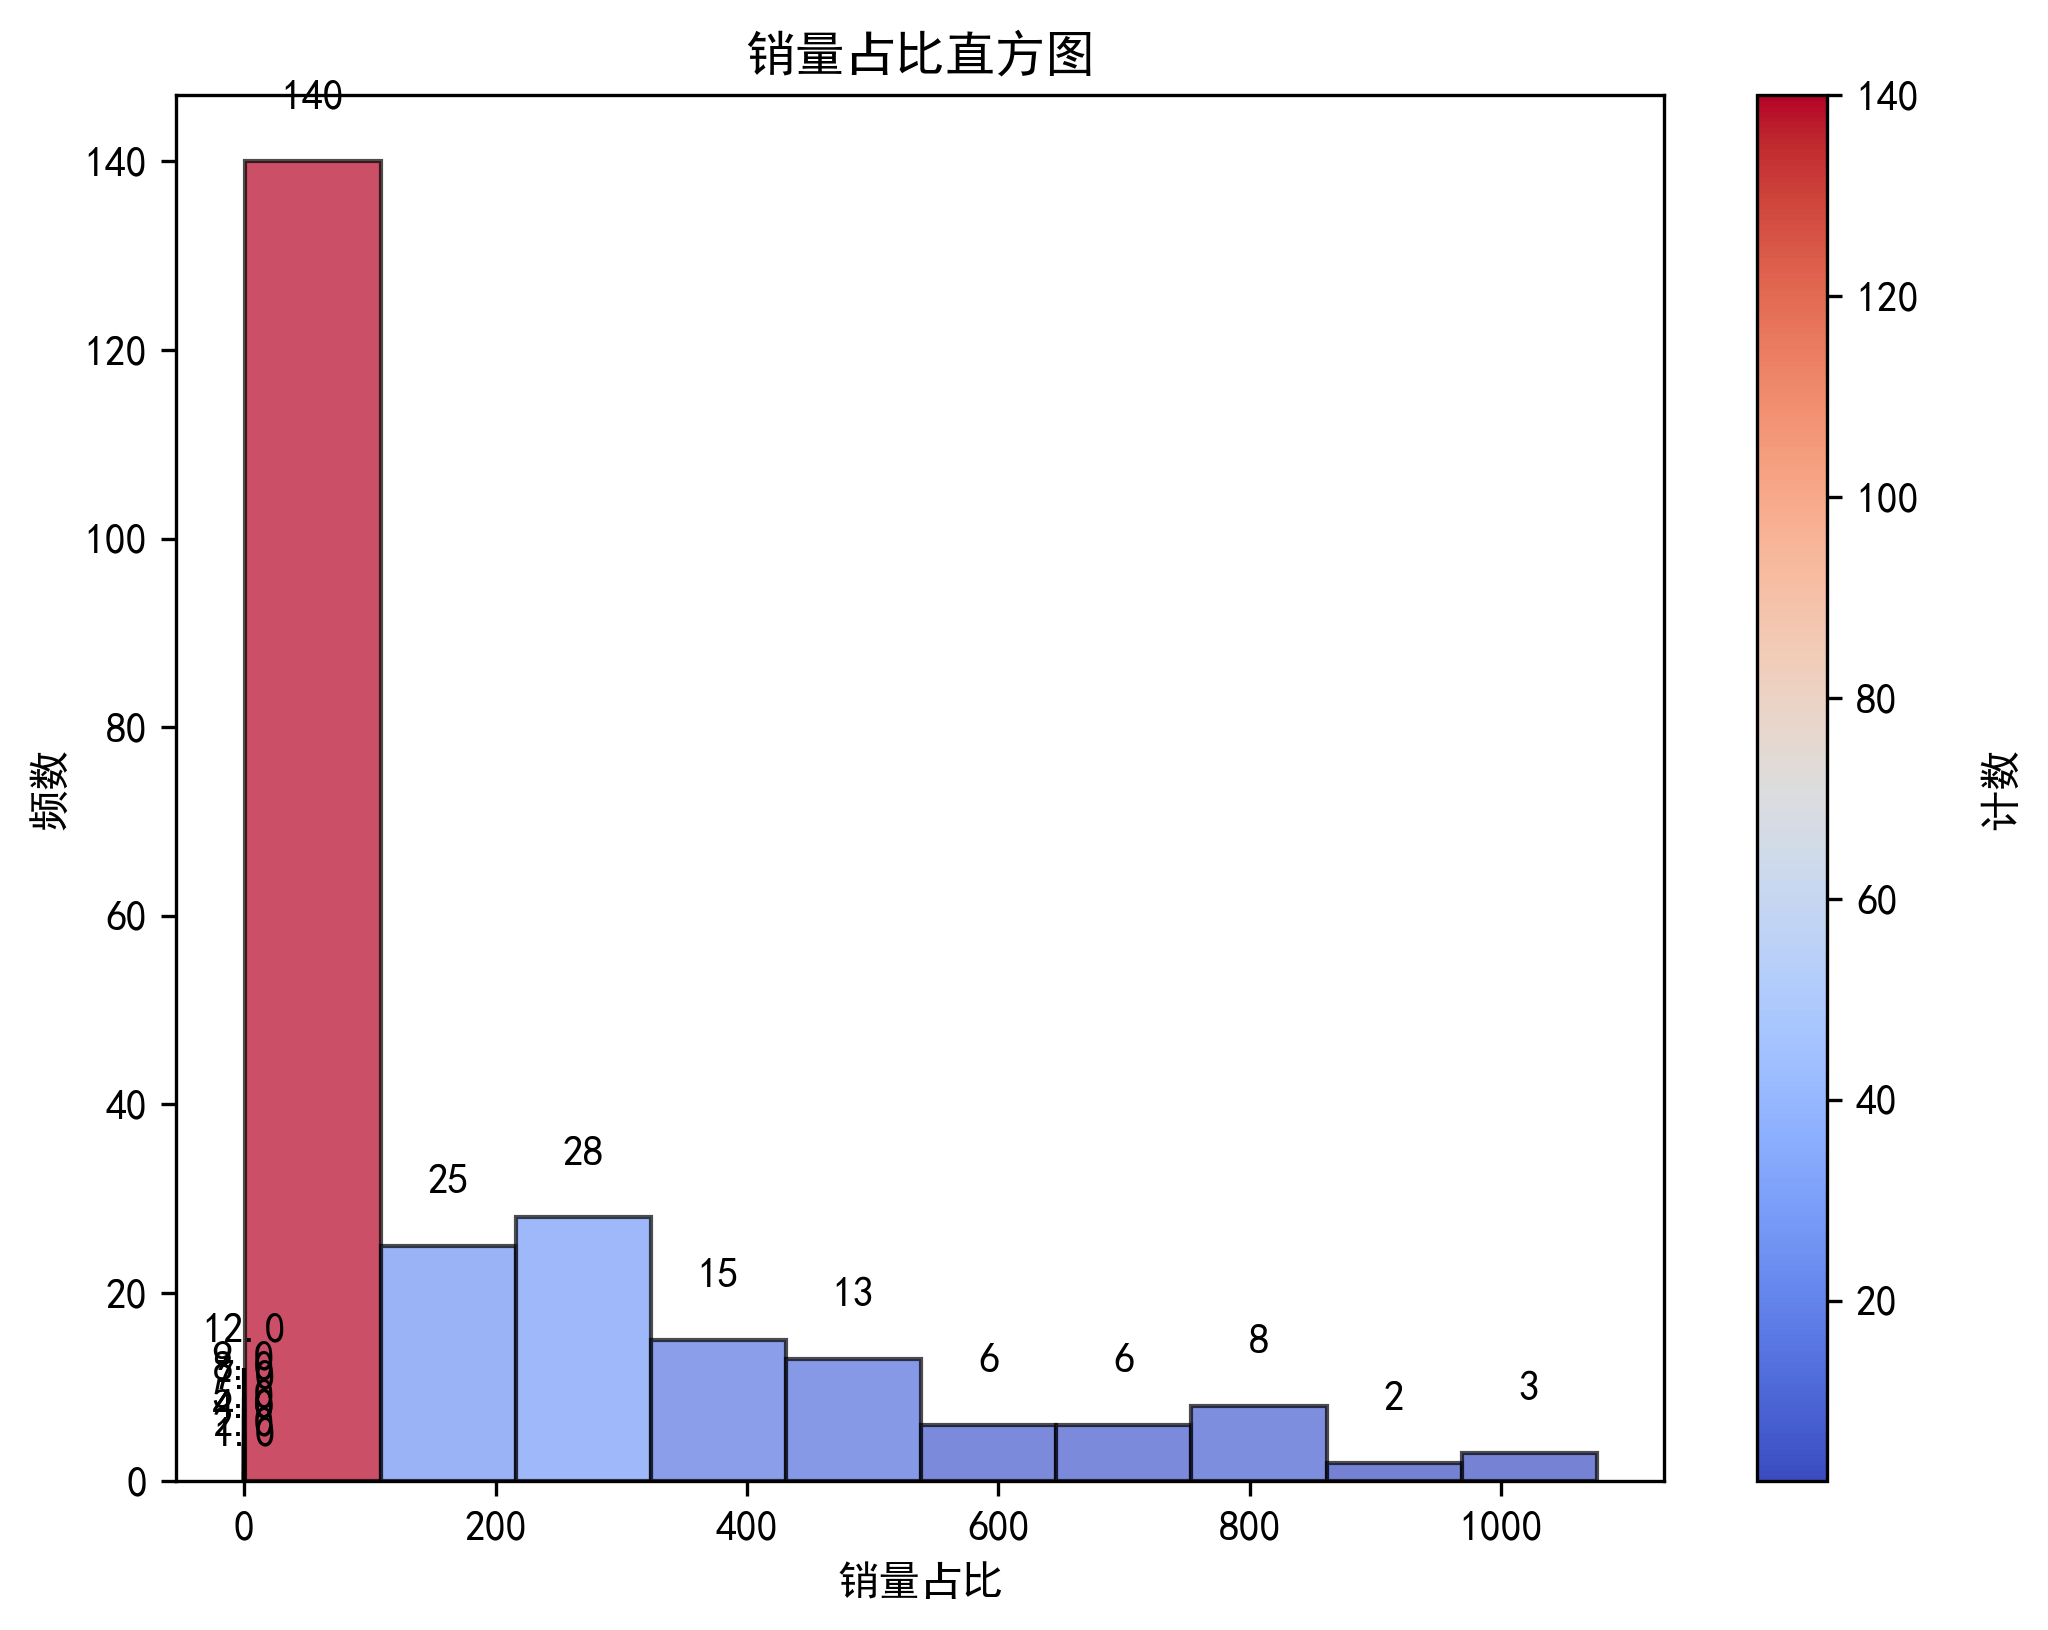
\includegraphics[width=0.95\textwidth]{销量占比直方图.png}
        \subcaption{销量占比直方图}
        \label{fig:sample-figure-b}
    \end{minipage}
    
    
    \label{fig:sample-figure}
\end{figure}
        \subsection{}
        \section{问题一模型的建立与求解}
        \subsection{基于自相关函数ACF的时间序列分析}
        \subsubsection{ACF的计算}
        $ACF(k)=\frac{Cov(y_t, y_{t-k})}{Var(y_t)}$，其中$k$为滞后阶数，$y_t$表示在$t$这个时间的观测数据，$y_{t-k}$表示在$t-k$这个时间的观测数据，$Cov$表示协方差，$Var$表示方差。
        \subsubsection{ACF图的绘制}
        根据ACF的计算结果，绘制ACF图，横轴为滞后天数，纵轴为自相关系数。
        \subsubsection{ACF图的解释}
        相关系数在滞后阶段0处为1，因为时间序列在同一个时间点上的值与自身的相关性始终是1。
        \newline
        若ACF图在之后的滞后阶段上有正相关性，则说明存在季节性。\newline 若ACF图在之后的滞后阶段上有负相关性，则说明存在反向季节性。\newline 若ACF图在之后的滞后阶段上基本为0，则说明基本无关。
        \subsection{时间分布规律的求解结果}
        \textbf{(a)各品类一年内月度销量的分布结果}
        各品类蔬菜三年平均的月度销售量变化如图1：
        \begin{figure}[!h]
    \centering
    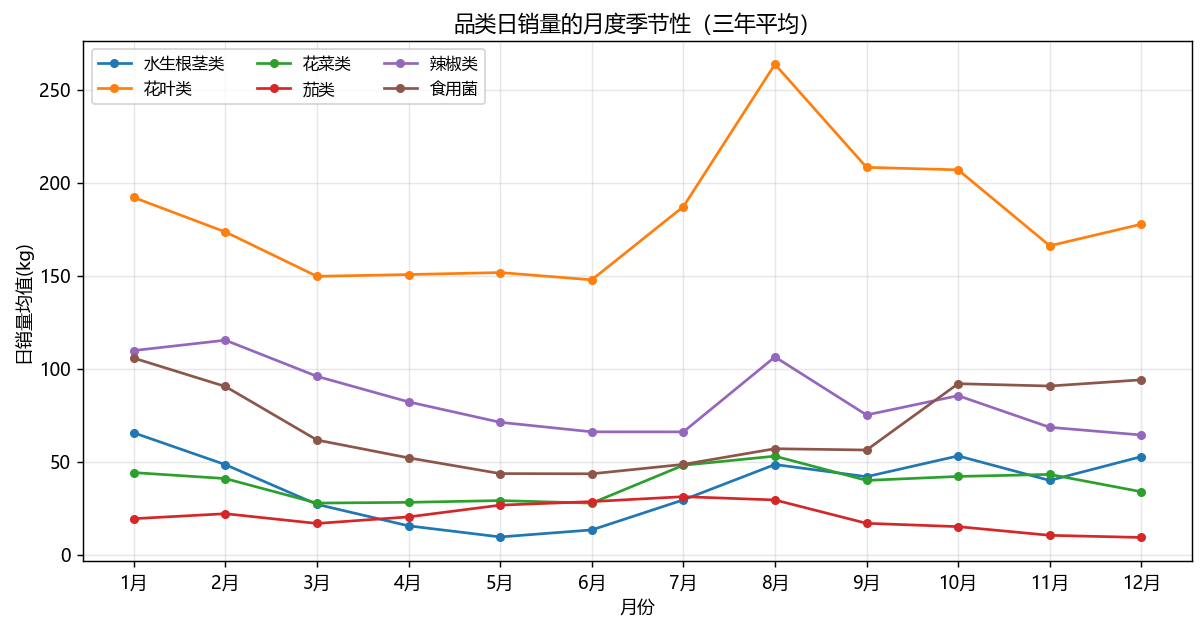
\includegraphics[width=0.8\linewidth]{a.png}
    \caption{一年各品类销售量变化图}
    \label{fig:circuit-diagram}
\end{figure}

考虑到蔬菜的产量受气候变化和节假日影响以及蔬菜的生长周期，因此以一个月为最小单位，分析各品类蔬菜销售量是否存在一年内的周期性变化。
\newline \hspace{2em}通过ACF图可以看出在与滞后阶段0相差12个月，通过观察图3，可以看出总销售量在春节和秋季会有大幅度增长，推测是由于春节期间人们采购年货和秋季农业丰收。 \newline
\textbf{(b)总销量一周内销量分布结果}
\begin{figure}[!h]
    \centering
    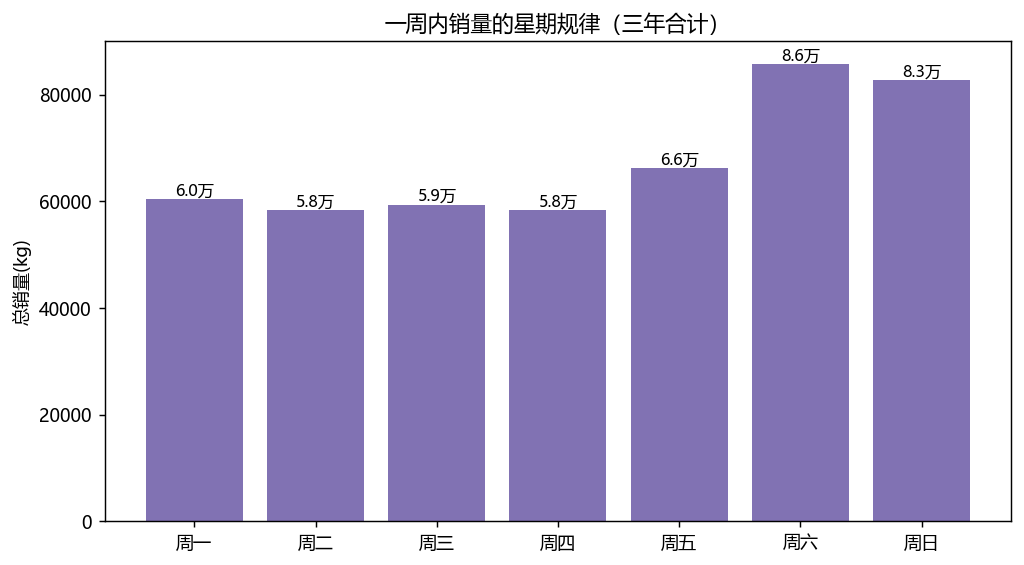
\includegraphics[width=0.8\linewidth]{一周内销量变化.png}
    \caption{一周内总销量变化图}
    \label{fig:circuit-diagram}
\end{figure}
由于人们工作是以周为单位，人们可能习惯将一周的蔬菜购买完，因此以一天为最小单位，分析总销量在一周内是否存在周期性变化的变化。\newline \hspace{2em} 分析一周内销量直方图，可以得到，每周一销量达到谷值，每周六销量达到峰值。这可能是因为人们习惯在结束一周的工作后将一周的蔬菜购买完，而工作日由于工作繁忙导致人们的购买欲望下降，蔬菜的销量在较低范围内波动。\newline
\subsection{销量分布规律的探究}
\subsubsection{销量占比}
绘出单品累计占比曲线如图可得，蔬菜高销售额单品只占少部分，大部分的商品销售量较低，前42个单品贡献了总销量的80\%，呈现明显的长尾分布。
\newline \hspace{2em} 各品类销售占比也存在较大差异，通过绘制各品类销量占比图如图5，发现花叶类销量占比最大，其次为辣椒类和食用菌，茄类销量占比最小。\newline \hspace{2em} 通过统计各品类品种丰富度，发现其与销量占比吻合，花叶类品种最为丰富，辣椒类和食用菌其次，茄类丰富度最低。
\begin{figure}[!h]
    \centering
    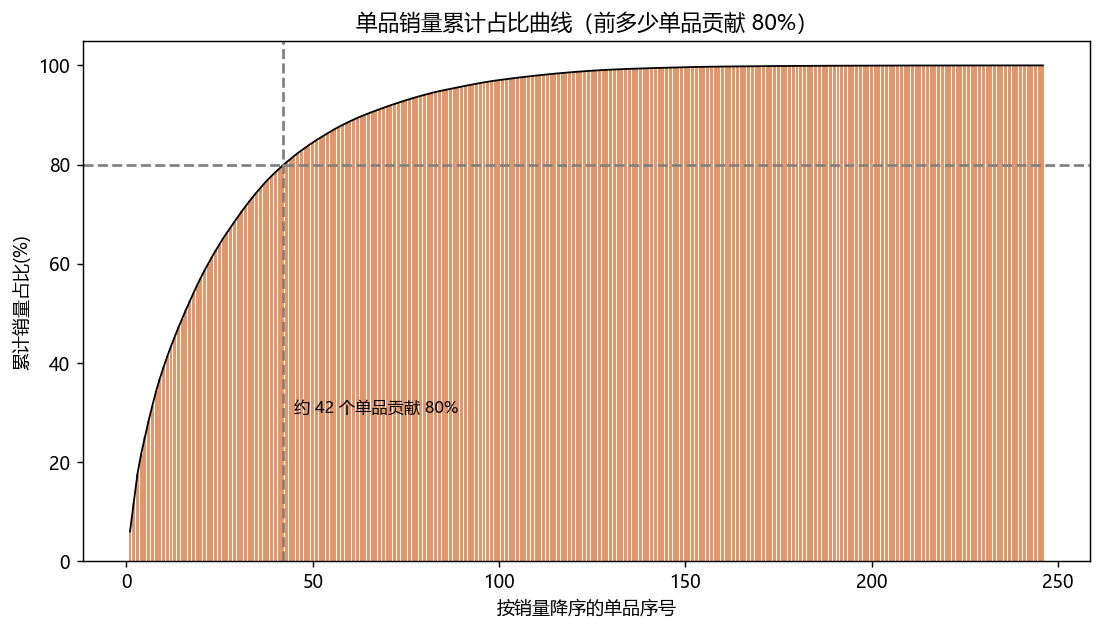
\includegraphics[width=0.8\linewidth]{销量占比.png}
    \caption{单品累计占比曲线}
    \label{fig:circuit-diagram}
\end{figure}
\begin{figure}[!h]
    \centering
    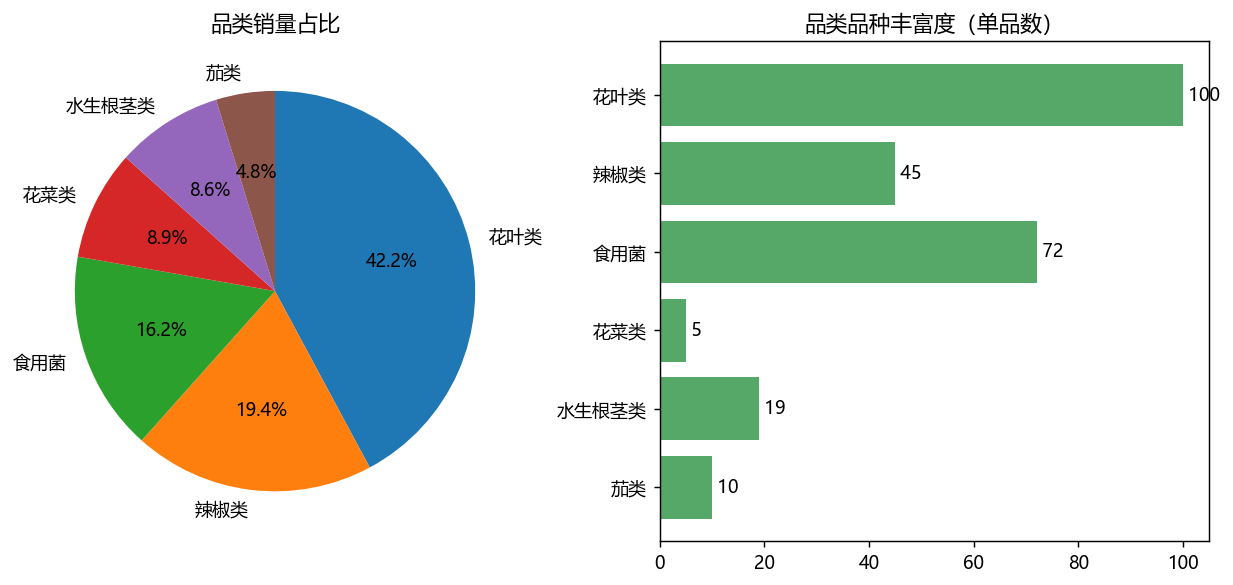
\includegraphics[width=0.8\linewidth]{各品类销售规律.png}
    \caption{各品类销量占比与品类品种丰富度}
    \label{fig:circuit-diagram}
\end{figure}
        \subsection{模型求解}
        \section{问题二模型的建立与求解} 
        \subsection{模型建立}
        \subsection{约束条件} 
        \subsection{模型求解}
        \section{问题三模型的建立与求解} 
        \subsection{模型建立}
        \subsection{约束条件} 
        \subsection{模型求解}
        \begin{equation}\tag{8}
            \sum_{j=16}^{\infty} x_{ijt} + \frac{\sum_{n=1}^{\infty} x_{ijt}}{2} \leq 1,\quad 27\leq i\leq 34
        \end{equation}
        \section{模型的评价、改进与推广}

        \begin{thebibliography}{9}%宽度9
            \bibitem{bib:one} ....
        \end{thebibliography}

        \begin{appendices}
        \section{数据预处理算法}
        \begin{lstlisting}[language=Python]
import pandas as pd
import matplotlib.pyplot as plt
plt.rcParams['font.sans-serif'] = [u'simHei']
plt.rcParams['axes.unicode_minus'] = False
csv_file = 'data/附件1.xlsx'
df_1 = pd.read_excel(csv_file)

csv_file = 'data/附件3.xlsx'
df = pd.read_excel(csv_file)
df['日期']= pd.to_datetime(df['日期'])
df['月份']= df['日期'].dt.month
#分品类
mapping_dict=df_1.set_index('单品编码')['分类名称'].to_dict()
df['品类']= df['单品编码'].map(mapping_dict)
print(df.head(5))

grouped=df.groupby('单品编码')
result={}

for name, group in grouped:
    unique_months = group['月份'].unique()
    total_months = len(unique_months)
    season = []
    season_list = [0] * 4
    if 3 in unique_months or 4 in unique_months or 5 in unique_months:
        season.append("春季")
        season_list[0] = 1
    if 6 in unique_months or 7 in unique_months or 8 in unique_months:
        season.append("夏季")
        season_list[1] = 1
    if 9 in unique_months or 10 in unique_months or 11 in unique_months:
        season.append("秋季")
        season_list[2] = 1
    if 12 in unique_months or 1 in unique_months or 2 in unique_months:
        season.append("冬季")
        season_list[3] = 1
    result[name] = {
        '出现的月份': unique_months,
        '总共出现的月份数': total_months,
        '出现的季节': season,
        "季节数": len(season),
        "季节列表": season_list
    }

count_all = 0
count_all_list = []
for key, value in result.items():
    if value['季节数'] == 4:
        count_all += 1
        count_all_list.append(key)

print(count_all)
print(count_all_list)
 \end{lstlisting}
        \end{appendices}
\end{document}